\documentclass[11pt]{article}
\usepackage{geometry}                % See geometry.pdf to learn the layout options. There are lots.
\geometry{letterpaper}                   % ... or a4paper or a5paper or ... 
%\geometry{landscape}                % Activate for for rotated page geometry
%\usepackage[parfill]{parskip}    % Activate to begin paragraphs with an empty line rather than an indent
\usepackage{graphicx}
\usepackage{amssymb}
\usepackage{slashed}
\usepackage{epstopdf}
\usepackage{amsmath}
\DeclareGraphicsRule{.tif}{png}{.png}{`convert #1 `dirname #1`/`basename #1 .tif`.png}

\setlength{\parindent}{0pt}

\usepackage{lmodern}
\usepackage{colortbl}

\usepackage{mmacells}
\usepackage{longtable}





\newcommand{\newc}{\newcommand}
\newcommand{\mychi}{\raisebox{0pt}[1ex][1ex]{\tiny$\chi$}}
\newcommand{\mychibig}{\raisebox{0pt}[1ex][1ex]{$\chi$}}

\newcommand{\chiinline}{\raisebox{1.7pt}[1ex][1ex]{$\chi$}}

\def\sp{\slashed{p}}
\def\sk{\slashed{k}}
\def\cn{\chi^0}
\def\cp{\chi^+}
\def\cm{\chi^-}
\def\gm{\gamma^{\mu}}
\def\gn{\gamma^{\nu}}
\def\gp{\gamma^{\rho}}
\def\km{k_{\mu}}
\def\kn{k_{\nu}}
\def\kp{k_{\rho}}
\renewcommand{\d}{\ensuremath{\operatorname{d}\!}}
\newc{\cTarasov}{a}


\def\cpp{\mychi^{++}}
\def\cmm{\mychi^{--}}
\def\Mp{M_{\text{pole}}}
\def\Mpa{M_{\text{pole},A}}
\def\Mpb{M_{\text{pole},B}}
\def\kmpm{k^{\mu}p_{\mu}}
\def\he{\frac{\epsilon}{2}}

\def\mc{m_{\mychi}}

\newcommand{\mb}{\textsf{Mass Builder} }
\newcommand{\mbs}{\textsf{Mass Builder}}
\newcommand{\tsil}{\textsf{TSIL} }
\newcommand{\tsils}{\textsf{TSIL}}
\newcommand{\tarcer}{\textsf{TARCER} }
\newcommand{\tarcers}{\textsf{TARCER}}
\newcommand{\sarah}{\textsf{SARAH} }
\newcommand{\sarahs}{\textsf{SARAH}}
\newcommand{\feynarts}{\textsf{FeynArts} }
\newcommand{\feynartss}{\textsf{FeynArts}}
\newcommand{\feyncalc}{\textsf{FeynCalc} }
\newcommand{\feyncalcs}{\textsf{FeynCalc}}

\newcommand{\mathematica}{\textsf{Mathematica} }
\newcommand{\CC}{C\nolinebreak\hspace{-.05em}\raisebox{.4ex}{\tiny\bf +}\nolinebreak\hspace{-.10em}\raisebox{.4ex}{\tiny\bf +} }

\usepackage{braket}

\begin{document}
\title{Radiative mass corrections in the vector dark matter model}
\maketitle
\section{Vector dark matter}

At the one-loop level we must consider interactions between the vector dark matter, the Higgs, the $W,Z$ and $\gamma$ gauge bosons and their goldstone bosons.  This gives 8 (12) one-loop diagrams for the neutral (charged) components of the vector dark matter.  These are given in Figures \ref{fig:1} and \ref{fig:2}.  The couplings we have are given in Table \ref{table:output_params}.

\begin{table}[h!]
\caption{The couplings involved and their assigned values.}\label{table:output_params}
\centering
\vspace{0.5cm}
\begin{tabular}{l l}
\hline
Parameter & Value \\
\hline
? ($a$) & 0.1\\
$SU(2)$ gauge coupling? ($EE$) & 0.1\\
? ($GG$) & 0.1 \\
\hline\end{tabular}
\end{table}

For vector fields the pole mass is given by
\begin{align}
M^+&=\sqrt{(\hat{M}^+)^2-\Pi(\hat{M}^+)}\\
M^0&=\sqrt{(\hat{M}^0)^2-\Pi(\hat{M}^0)}
\end{align}
where $\hat{M}^+$ and $\hat{M}^0$ are the ``tree-level" MS bar masses of the charged and neutral components of the triplet dark matter respectively.\\

In Figure \ref{fig:mass_splittings} I show the mass splitting for two fixed values of the renormalisation scale.  As we can see the mass splitting reaches a fixed value which is, as expected, independent of the tree-level mass and the renormalisation scale.  This is because, if one was to compare the results analytically, the difference of the self energies would not contain any functional dependence on $\mu$ or $M$.  While this is trivial to show by hand in a fermionic $SU(2)$ multiplet, the task is somewhat more cumbersome to do for a vector triplet as we have many more diagrams to consider.  Fortunately, the result is evident from our numerical analysis.

\begin{figure}[h]
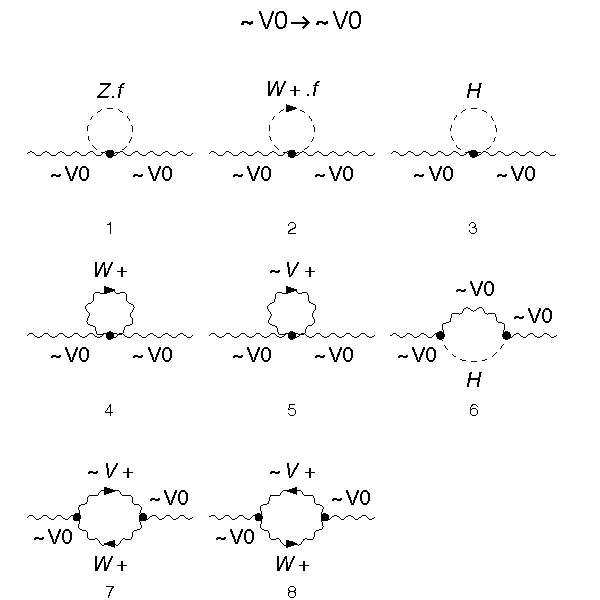
\includegraphics[width=0.5\textwidth]{diagrams_V[6]_1.pdf}\\
\caption{One-loop radiative mass corrections for the neutral component.}\label{fig:1}
\end{figure}
\begin{figure}[h]
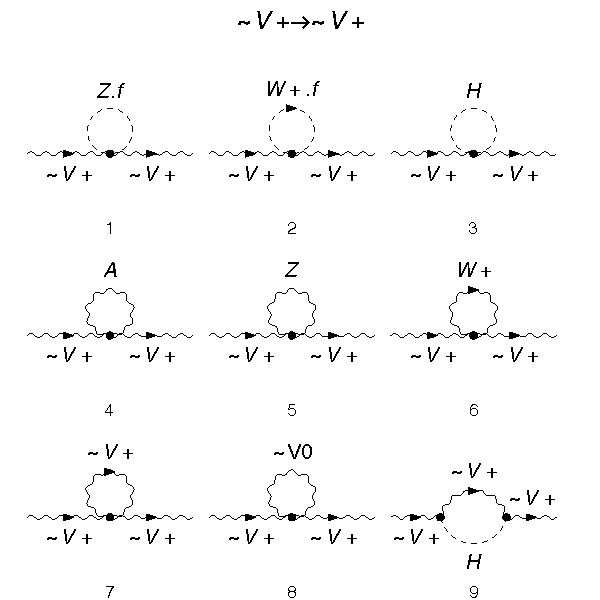
\includegraphics[width=0.5\textwidth]{diagrams_V[5]_1_1.pdf}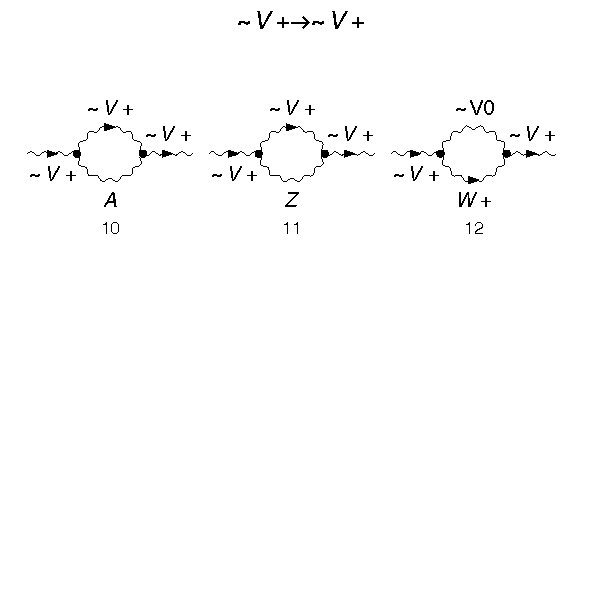
\includegraphics[width=0.5\textwidth]{diagrams_V[5]_1_2.pdf}
\caption{One-loop radiative mass corrections for the charged component.}\label{fig:2}
\end{figure}


\begin{figure}[h]
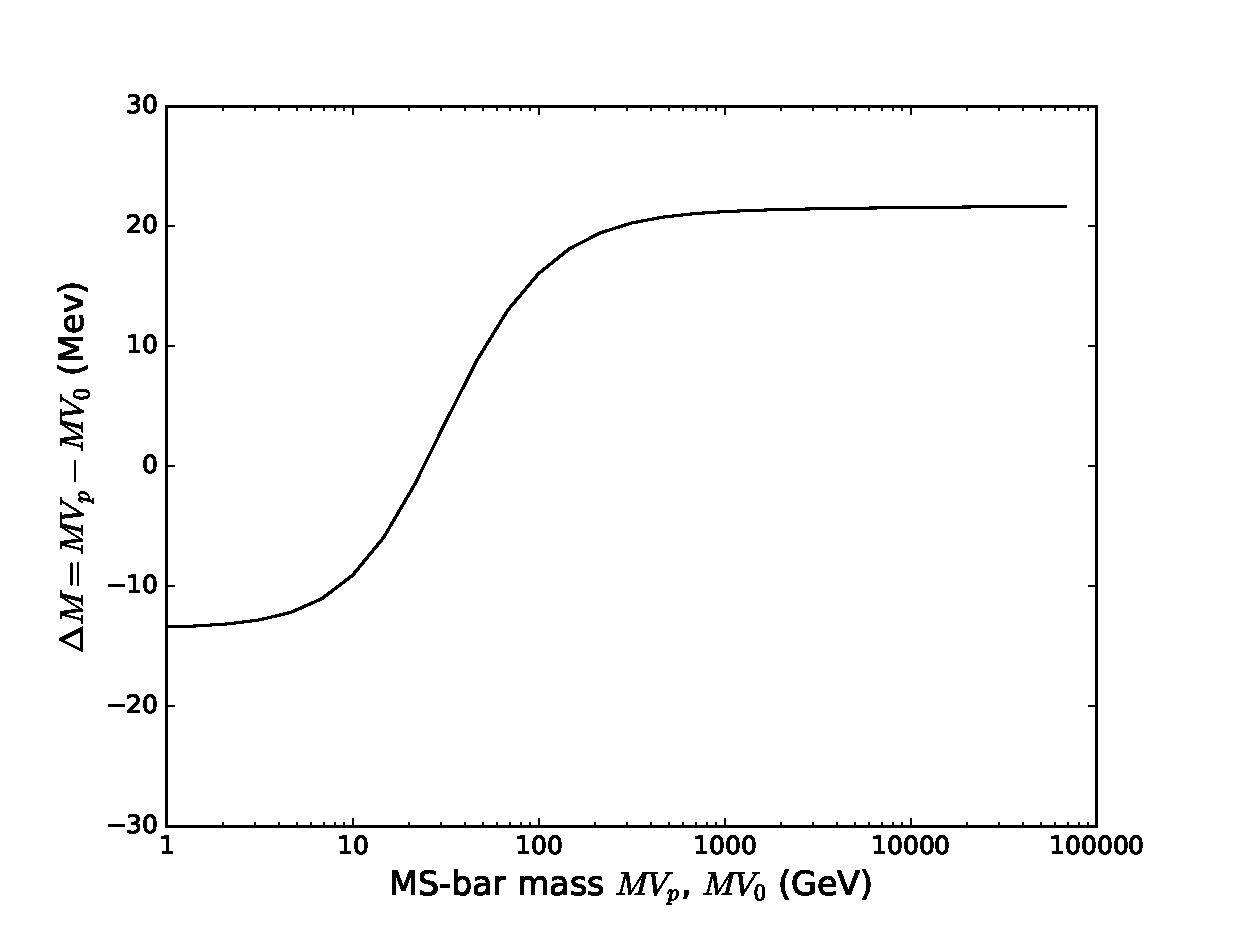
\includegraphics[width=0.5\textwidth]{mass_splittings.eps}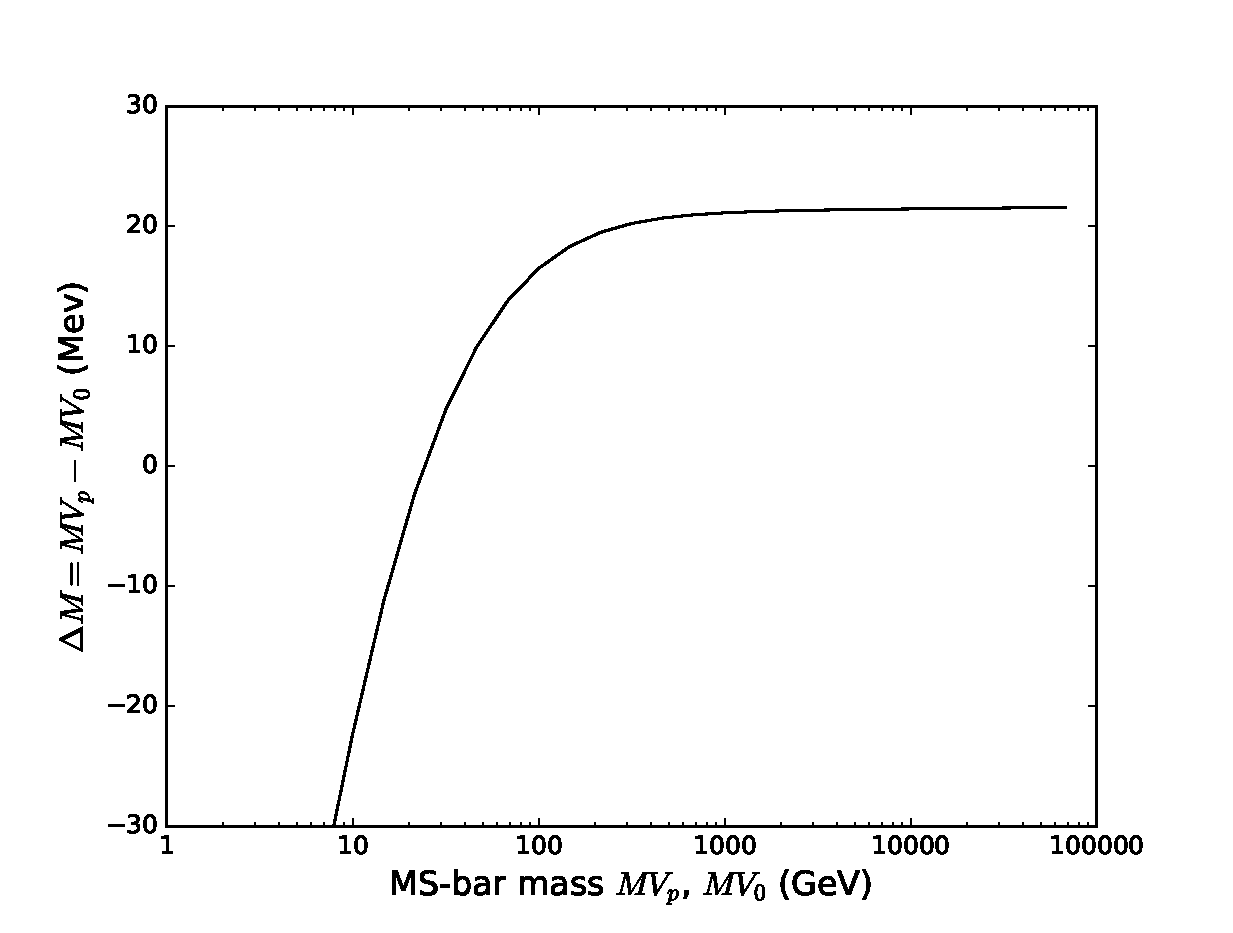
\includegraphics[width=0.5\textwidth]{mass_splittings_5k.eps}\\
\caption{Mass splitting between components of vector dark matter using fixed renormalisation scale $\mu=100$ GeV (\textit{left}) and $\mu=5000$ GeV (\textit{right}) and parameters as given in Table \ref{table:output_params}.  It is evident that $\mu=5000$ GeV is not an appropriate choice for low mass calculations!} \label{fig:mass_splittings}
\end{figure}



\bibliography{../../../../Papers/library}{}
\bibliographystyle{science}

\end{document}  